\chapter{Struktur der Software \dcsecondauthorshort}
\label{cha:software_struktur}
Dieses Kapitel legt das Zusammenspiel der verwendeten Software-Komponenten dar. Es wird auf die Nutzung vorhandener \gls{acr:ros}-Komponenten sowie die Umsetzung der eigens implementierten Echtzeitanwendung mit MATLAB eingegangen.

\section{ROS \dcsecondauthorshort}
Da der Austausch von Bilddaten und Ansteuerbefehlen zwischen Modellfahrzeug und PC via \gls{acr:ros}\footnote{http://www.ros.org/} abläuft, soll kurz darauf eingegangen werden. 
\begin{quotation}
\gls{acr:ros} ist eine Sammlung von Werkzeugen, Bibliotheken und Konventionen zur Vereinfachung der Entwicklung komplexen und robusten Roboterverhaltens für eine Vielzahl an Roboterplattformen.\footnote{Übernommen aus dem Englischen von http://www.ros.org/about-ros/ am 11. September 2018}
\end{quotation}

%\subsection{Nodes}
\label{ssec:software_struktur:ros:nodes}
\ \\
Ein \gls{acr:ros}-System besteht aus mehreren Programmen (\glqq Nodes\grqq ), welche über bestimmte Kommunikationskanäle (\glqq Topics\grqq ) Datenpakete (\glqq Messages\grqq ) austauschen. Diese Applikationen können als sogenannte Publisher Informationen auf einem Topic zur Verfügung stellen. Im anderen Fall man nennt sie Subscriber, wenn sie stattdessen Informationen nutzen. Ein Schema zum Aufbau des konkreten \gls{acr:ros}-Systems findet sich in Abb.~\ref{fig:software_struktur:ros}.

\begin{figure}[htbp]
	\centering
	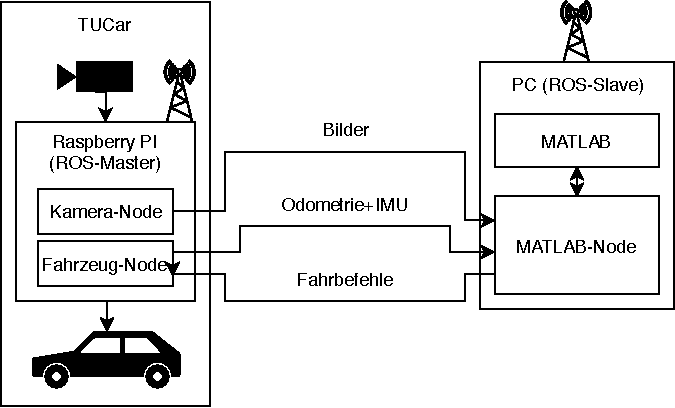
\includegraphics[width=1.0\textwidth]{Software_Struktur_ROS}
	\caption{Struktur des ROS-Systems}
	\label{fig:software_struktur:ros}
\end{figure}

%\subsubsection{Fahrzeug}
\paragraph{Kamera-Node}
Der Kamera-Node veröffentlicht die Bilder als Rohdaten-Topic sowie in komprimierter Form.
\paragraph{Fahrzeug-Node}
Der Fahrzeug-Node veröffentlicht:
\begin{itemize}
\item Odometriedaten 
\item Messwerte der \gls{acr:imu}
\item sonstige Informationen zum Fahrzeug (z.B. Akkuspannung)
\end{itemize}
und nimmt im Ansteuer-Topic die gewünschte Geschwindigkeit und den Lenkwinkel entgegen.
\paragraph{PC}
Auf dem PC wird nur der von MATLAB automatisch initialisierte Node genutzt. Dieser abonniert das komprimierte Bilddaten-Topic und veröffentlicht auf das Ansteuer-Topic des Fahrzeugs.

\section{MATLAB \dcsecondauthorshort}
Die im Hauptteil dieser Arbeit beschriebenen Algorithmen zur Fahrspurverfolgung wurden ausschließlich in MATLAB implementiert. \textbf{MAT}rix \textbf{LAB}oratory ist ein kommerzielles Programm und eine Programmiersprache für numerische Rechnungen und grafische Darstellungen, dessen Grundbausteine Matrizen sind. Diese Eigenschaften, weitreichende Debugging-Funktionalitäten und die einfache Erweiterbarkeit durch sogenannte Toolboxen machen es sehr attraktiv zum Einsatz im Rahmen der Bildverarbeitung \& Evaluation. Da die grundlegende Softwarestruktur in allen drei Lösungsansätzen zur Fahrspurverfolgung gleich ist, soll diese nun dargelegt werden. Eine schematische Darstellung ist in Abb.~\ref{fig:software_struktur:matlab} gegeben.

\begin{figure}[htbp]
	\centering
	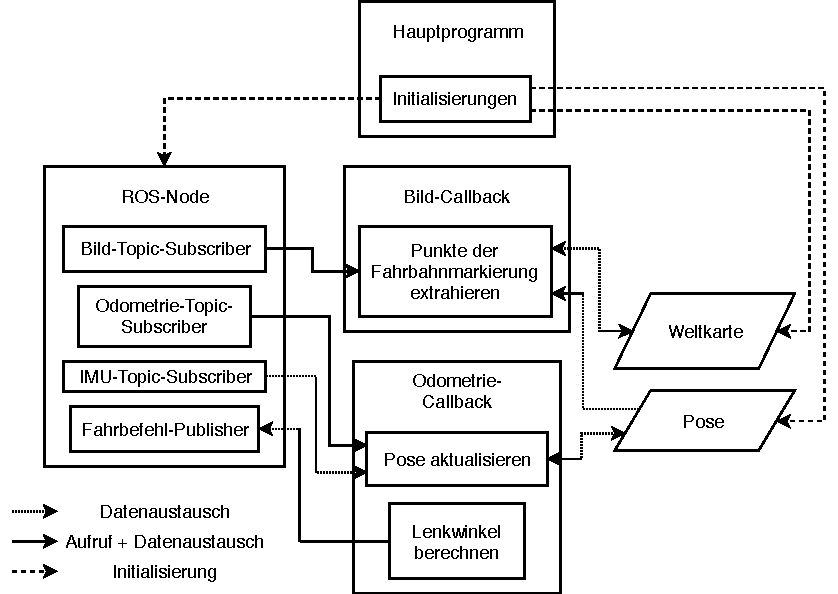
\includegraphics[width=1.0\textwidth]{Software_Struktur_Matlab}
	\caption{Struktur des MATLAB-Softwareteils}
	\label{fig:software_struktur:matlab}
\end{figure}

\subsection{Initialisierung}
Ist das Fahrzeug betriebsbereit, d.h. werden alle Nodes des Fahrzeugs ausgeführt, so kann in MATLAB das Programm zur Fahrspurverfolgung aufgerufen werden. Hierfür wird die Initialisierungsroutine gestartet welche:
\begin{itemize}
\item die globalen Parameter lädt
\item die Weltkarte und die Pose initialisiert
\item den MATLAB-\gls{acr:ros}-Node startet
\item die Subscriber des Bilddaten-, Odometrie- und \gls{acr:imu}-Topics anlegt
\item eine konstante tangentiale Geschwindigkeit des Fahrzeugs vorgibt 
\end{itemize}

\subsection{Callbacks}
\label{ssec:software_struktur:matlab:callbacks}
Sind alle Startroutinen abgeschlossen, so werden Programmteile nur noch eventbasiert in sogenannten Callback-Funktionen ausgeführt.
 
\paragraph{Odometrie-Callback}
Das Fahrzeug veröffentlicht in konfigurierbaren Abständen seine aktuellen Odometriedaten.
Das Eintreffen eines solchen Datenpaketes in MATLAB führt zum Aufrufen der Odometrie-Callback-Funktion. Die Hauptaufgabe dieses Programmteils besteht in der Regelung des Fahrzeugs, deren Ablauf im folgenden kurz erläutert wird.
\begin{enumerate}
\item Mithilfe der empfangenen, seit der letzten Odometrie-Message verstrichenen Zeit, der in dieser Spanne ermittelten Durchschnittsgeschwindigkeit und der durch die \gls{acr:imu} erhaltenen Orientierung kann die Pose aktualisiert werden. Vorherige Posen werden inklusive des Zeitstempels der sie generierenden Odometrie-Daten für den im Folgenden erläuterten Bild-Callback abgespeichert.
\item Auf Basis der neuen Pose kann mithilfe aller in der Weltkarte vorhandenen Punkte ein neuer Lenkwinkel bestimmt werden.
\end{enumerate}
\paragraph{Bild-Callback}
Sobald ein neues Bild im zugehörigen Topic verfügbar ist, wird ein Algorithmus zur Extraktion von Punkten der Fahrbahnmarkierung gerufen. Dieser fügt die gefundenen Koordinatenserien anhand der am besten zum Aufnahmezeitpunkt des Bildes passenden Pose nach Linientyp sortiert (\glqq linke\grqq , \glqq mittlere\grqq{} oder \glqq rechte\grqq{} Linie) in die Weltkarte ein und macht sie so für die Regelung abrufbar.

Eine ausführlichere Erläuterung zur Wirkungsweise und zu Vorteilen einer Aufteilung von Bildverarbeitung und Regelung in mehrere Callback-Funktionen ist in Abschnitt \ref{sec:regelung:implementierung} gegeben.
\subsection{Multitasking}
Da MATLAB ohne spezielle Toolboxen Prozesse nicht gleichzeitig ausführen kann, die Bearbeitungszeit eines Bild-Callbacks jedoch wesentlich länger ist als die angestrebte Periodendauer der Regelung (Häufigkeit des Aufrufs eines Odometrie-Callbacks), musste für eine Unterbrechbarkeit der Bildverarbeitung gesorgt werden. MATLAB reagiert bei der Ausführung eines Tasks nur während bestimmter Befehle auf weitere Ereignisse. Eine Möglichkeit die Regelung auch bei noch nicht vollständig ausgeführtem Bild-Callback zu ermöglichen, besteht im Einfügen kurzer Pausen zwischen Programmteilen zur Segmentierung dessen. Wählt man diese Abschnitte hinreichend kurz, kann der wartende Odometrie-Callback mit wenig Verzögerung ausgeführt und die Bildverarbeitung danach fortgesetzt werden.


